\documentclass[twocolumn,aps,prd,nofootinbib,superscriptaddress,10pt,notitlepage,preprintnumbers] {revtex4-1} 
\usepackage{amssymb,amsmath,verbatim,mathtools,needspace,enumitem,etoolbox,graphicx}
%\usepackage[dvipsnames, usenames]{xcolor}
\usepackage{tcolorbox}
\definecolor{linkcolor}{rgb}{0.0,0.3,0.5}
\usepackage[unicode, colorlinks=true, linkcolor=linkcolor, citecolor=linkcolor, filecolor=linkcolor,urlcolor=linkcolor, pdfusetitle]{hyperref}
\usepackage{epstopdf}

\usepackage{bm}
\usepackage{dcolumn}
\usepackage[utf8]{inputenc} 
\usepackage{latexsym}
\usepackage{rotating}
\usepackage{color}
\usepackage{xcolor}
\usepackage{enumerate}
\usepackage{mathtools}
\usepackage{url}
\definecolor{ocre}{RGB}{100,134,158}

\setlength{\tabcolsep}{12pt}
\newcommand{\red}[1]{\textcolor{red}{#1}}

\newcommand{\tn}{\textnormal}
\newcommand{\bss}[1]{\textcolor{red}{[\sf{BSS: #1}]}}
\newcommand{\pnp}[1]{\textcolor{blue}{#1}}

\begin{document}
\title{What next for gravitational wave astronomy?}

\author{B. S. Sathyaprakash} % \email{bss25@psu.edu}
\affiliation{Institute for Gravitation and the Cosmos, Department of Physics, Penn State University,
University Park PA 16802, USA}
\affiliation{Department of Astronomy and Astrophysics, Penn State University, University Park PA 16802, USA}
\affiliation{School of Physics and Astronomy, Cardiff University, Cardiff, CF24 3AA, United Kingdom}
\author{Matthew Evans}
\affiliation{Department of Physics, Massachusetts Institute of Technology, Cambridge MA 02139, USA}
\begin{abstract}
\end{abstract}
\maketitle
\subsection*{Discovery of a Lifetime}
Observation of gravitational waves (GWs) from black hole binaries by the Laser Interferometer Gravitational-Wave Observatory (LIGO) on September 14, 2015 \cite{GW150914} was a momentous occasion in the history of physics.  The observation finally verified a key prediction of general relativity (GR) that Albert Einstein \cite{Einstein:1915ca,Einstein:1918btx} had made a century earlier and laid to rest a quest that began with the experiments of Joseph Weber \cite{Weber:1960zz} in the sixties. 

Two years later, in August 2017, LIGO and the European Virgo made another landmark discovery, this time the inspiral and coalescence of a pair of neutron stars \cite{GW170817}. The collision produced a powerful jet of gamma rays that was observed a mere two seconds later by the Fermi Gamma-ray Space Telescope \cite{GW-GRB170817}. X-ray, UV, Optical, infrared and radio telescopes around the world and in space watched the fireworks produced in the aftermath of the collision in the entire electromagnetic window \cite{GBM:2017lvd}. That was a watershed moment in astronomy, ushering in a new era in multimessenger astronomy.

In the past four years, LIGO and Virgo have continued to make spectacular discoveries \cite{LIGOScientific:2019fpa} of new classes of sources \cite{Abbott:2020uma, LIGOScientific:2020stg} and provided a treasure trove of data that has not only transformed our understanding in some areas of physics and astronomy but shaking established wisdom in others. Yet this is only the beginning.  In this article we will describe a sample of the exciting new results brought to bear by current observations and how future observatories could uniquely explore some of the outstanding problems in physics and astronomy.

\begin{figure} [bh]
%\begin{tcolorbox}[standard jigsaw, colframe=gray,colback=black!10!cyan,opacityback=0.1,coltext=black,title=\sc Science Goals for Next Generation Ground-Based Detectors]
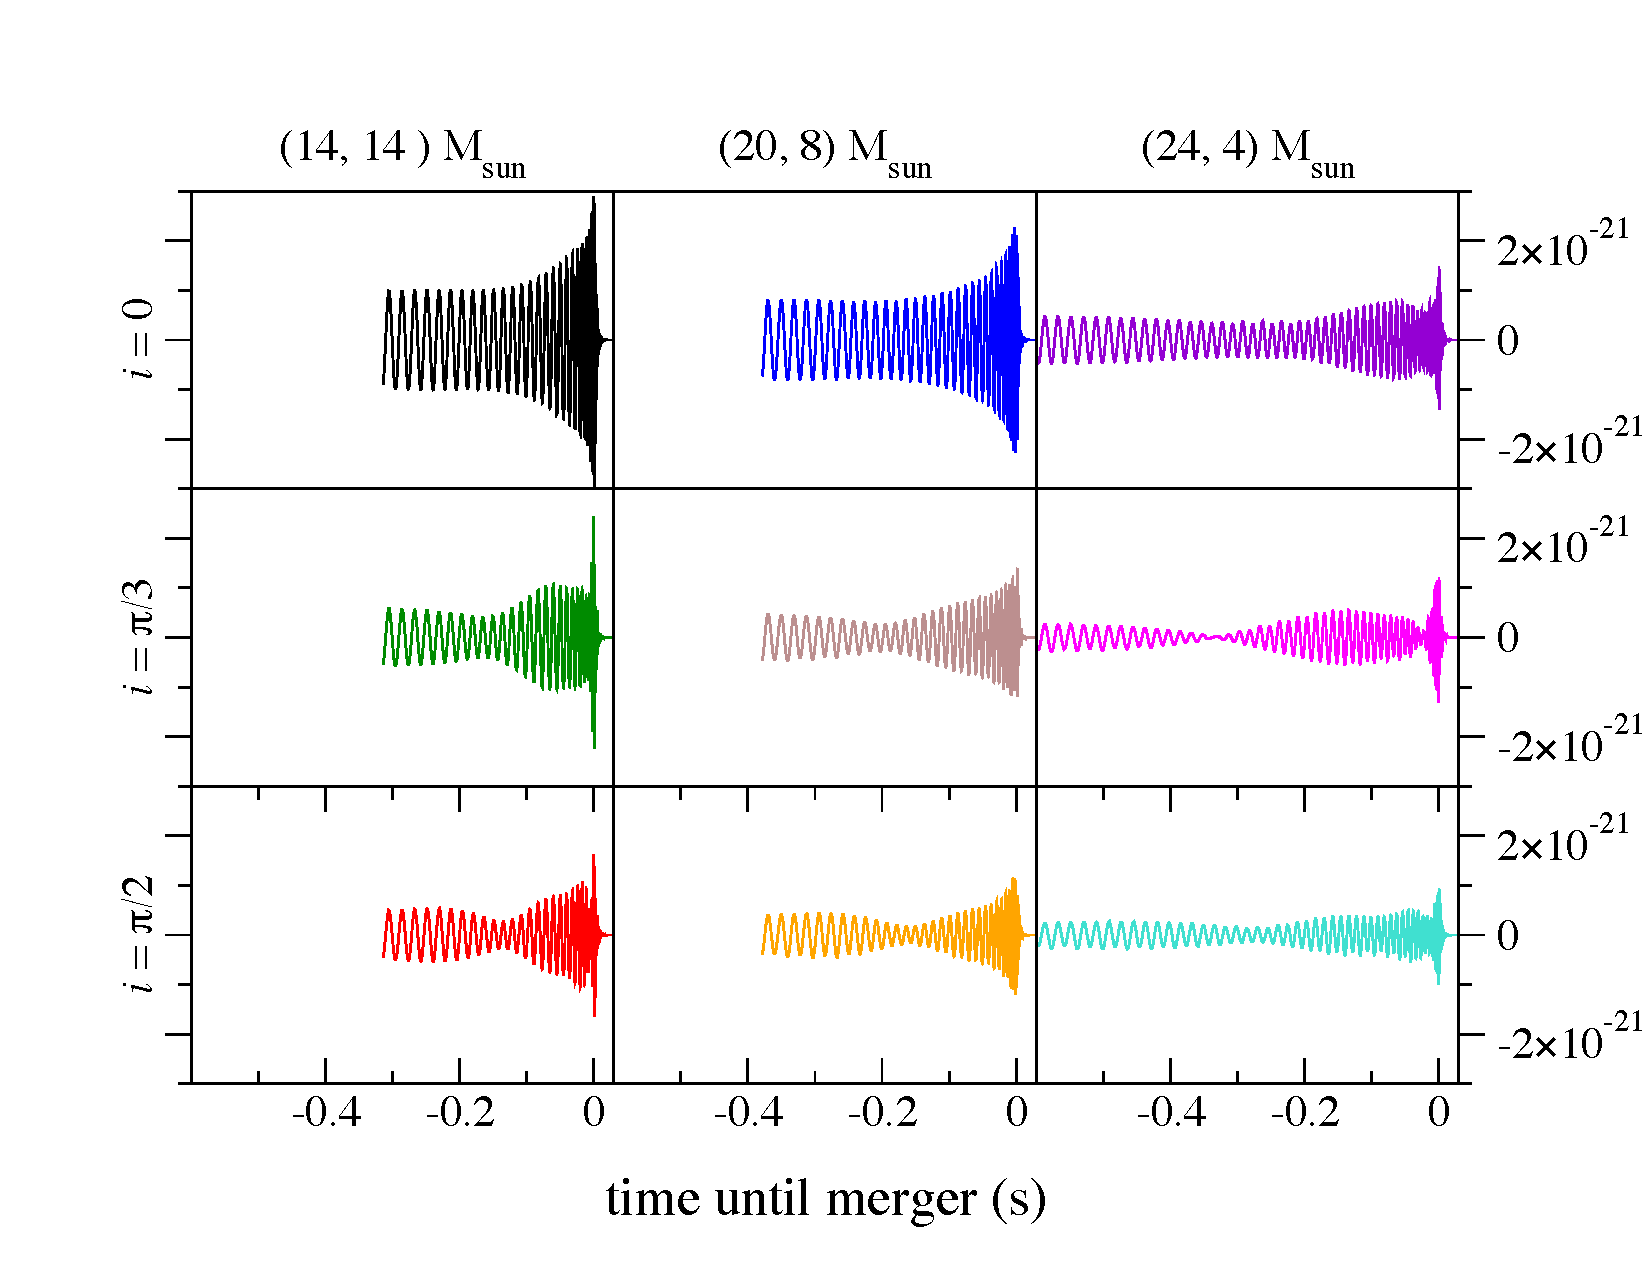
\includegraphics[width=0.505\textwidth]{wavezoov2.pdf}
\caption{Zoo of waveforms from binary black holes, all starting at the same initial frequency of 50 Hz and of the same total mass of $28M_\odot.$ Both black holes have the same dimensionless spin of $c{\mathbf S}_{1,2} / Gm_{1,2}^2 = (0.7,0,0.6),$ and orbital angular momentum along the $z$ axis. The diagram illustrates how the amplitude of the waveform, its length and its modulation depends on the companion masses and the viewing angle $\iota$.}
\label{fig:wavezoo}
%\end{tcolorbox}
\vskip-0.5cm
\end{figure}

\subsection*{\bf A New Era in Fundamental Physics \& Astronomy}
Compact binaries are the reason why interferometric detectors were built. Today, they are the only sources that have been confidently detected. Their discovery, and the extraction of the exquisite science that ensues, has been possible thanks to the availability of highly accurate analytical \cite{Blanchet:1994ez, Buonanno:2000ef, Ajith:2009bn} and numerical \cite{Pretorius:2005gq, Campanelli:2005dd, Baker:2005vv} solutions to the two-body in GR. Figure \ref{fig:wavezoo} lists a sample of waveforms from binaries to show how the shape and duration of the signals depend on the parameters of the binary. This accurate knowledge of the waveforms is exploited to pull the signals out of noise using matched filtering \cite{Sathyaprakash:1991mt} and to reconstruct the parameters of the signal and the source. To fully reconstruct the wave, it is necessary to observe the signal in a network of three or more non-collocated detectors \cite{Sathyaprakash:2009xs}. Thus, science was the big motivation why observatories around the world began data sharing from the word go and why future detectors would need to do the same for getting the maximum science out of GW data. 

LIGO/Virgo observations made during their first and second observing runs are already transforming the field of fundamental physics and have provided invaluable data on decades old problems in astronomy. In addition to GW150914, LIGO and Virgo have discovered entirely new classes of systems that include GW170817 (a coalescing neutron star binary) \cite{GW170817}, GW190521 (a black hole binary whose primary companion has mass in excess of $60\,M_\odot$) \cite{}, and GW190814 (a system with a mass ratio of 1:10 that hosts the lightest  black hole or the heaviest neutron star) \cite{}. The most impactful conclusions from these discoveries are:

\begin{figure*} 
%\begin{tcolorbox}[standard jigsaw,colframe=gray,colback=black!10!cyan,opacityback=0.1,coltext=black,title=\sc Science Goals for Next Generation Ground-Based Detectors]
\fbox{
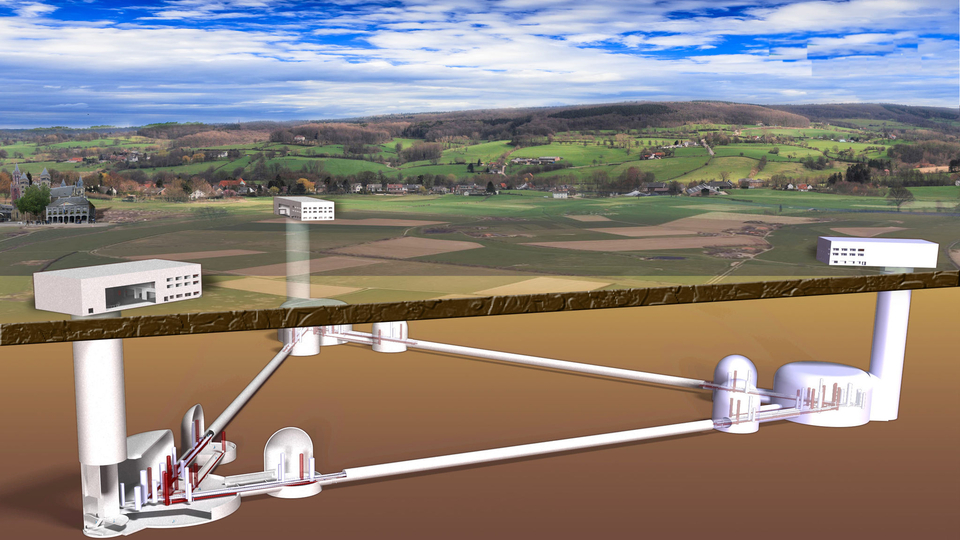
\includegraphics[width=0.48\textwidth]{ET-Netherlands.jpg}
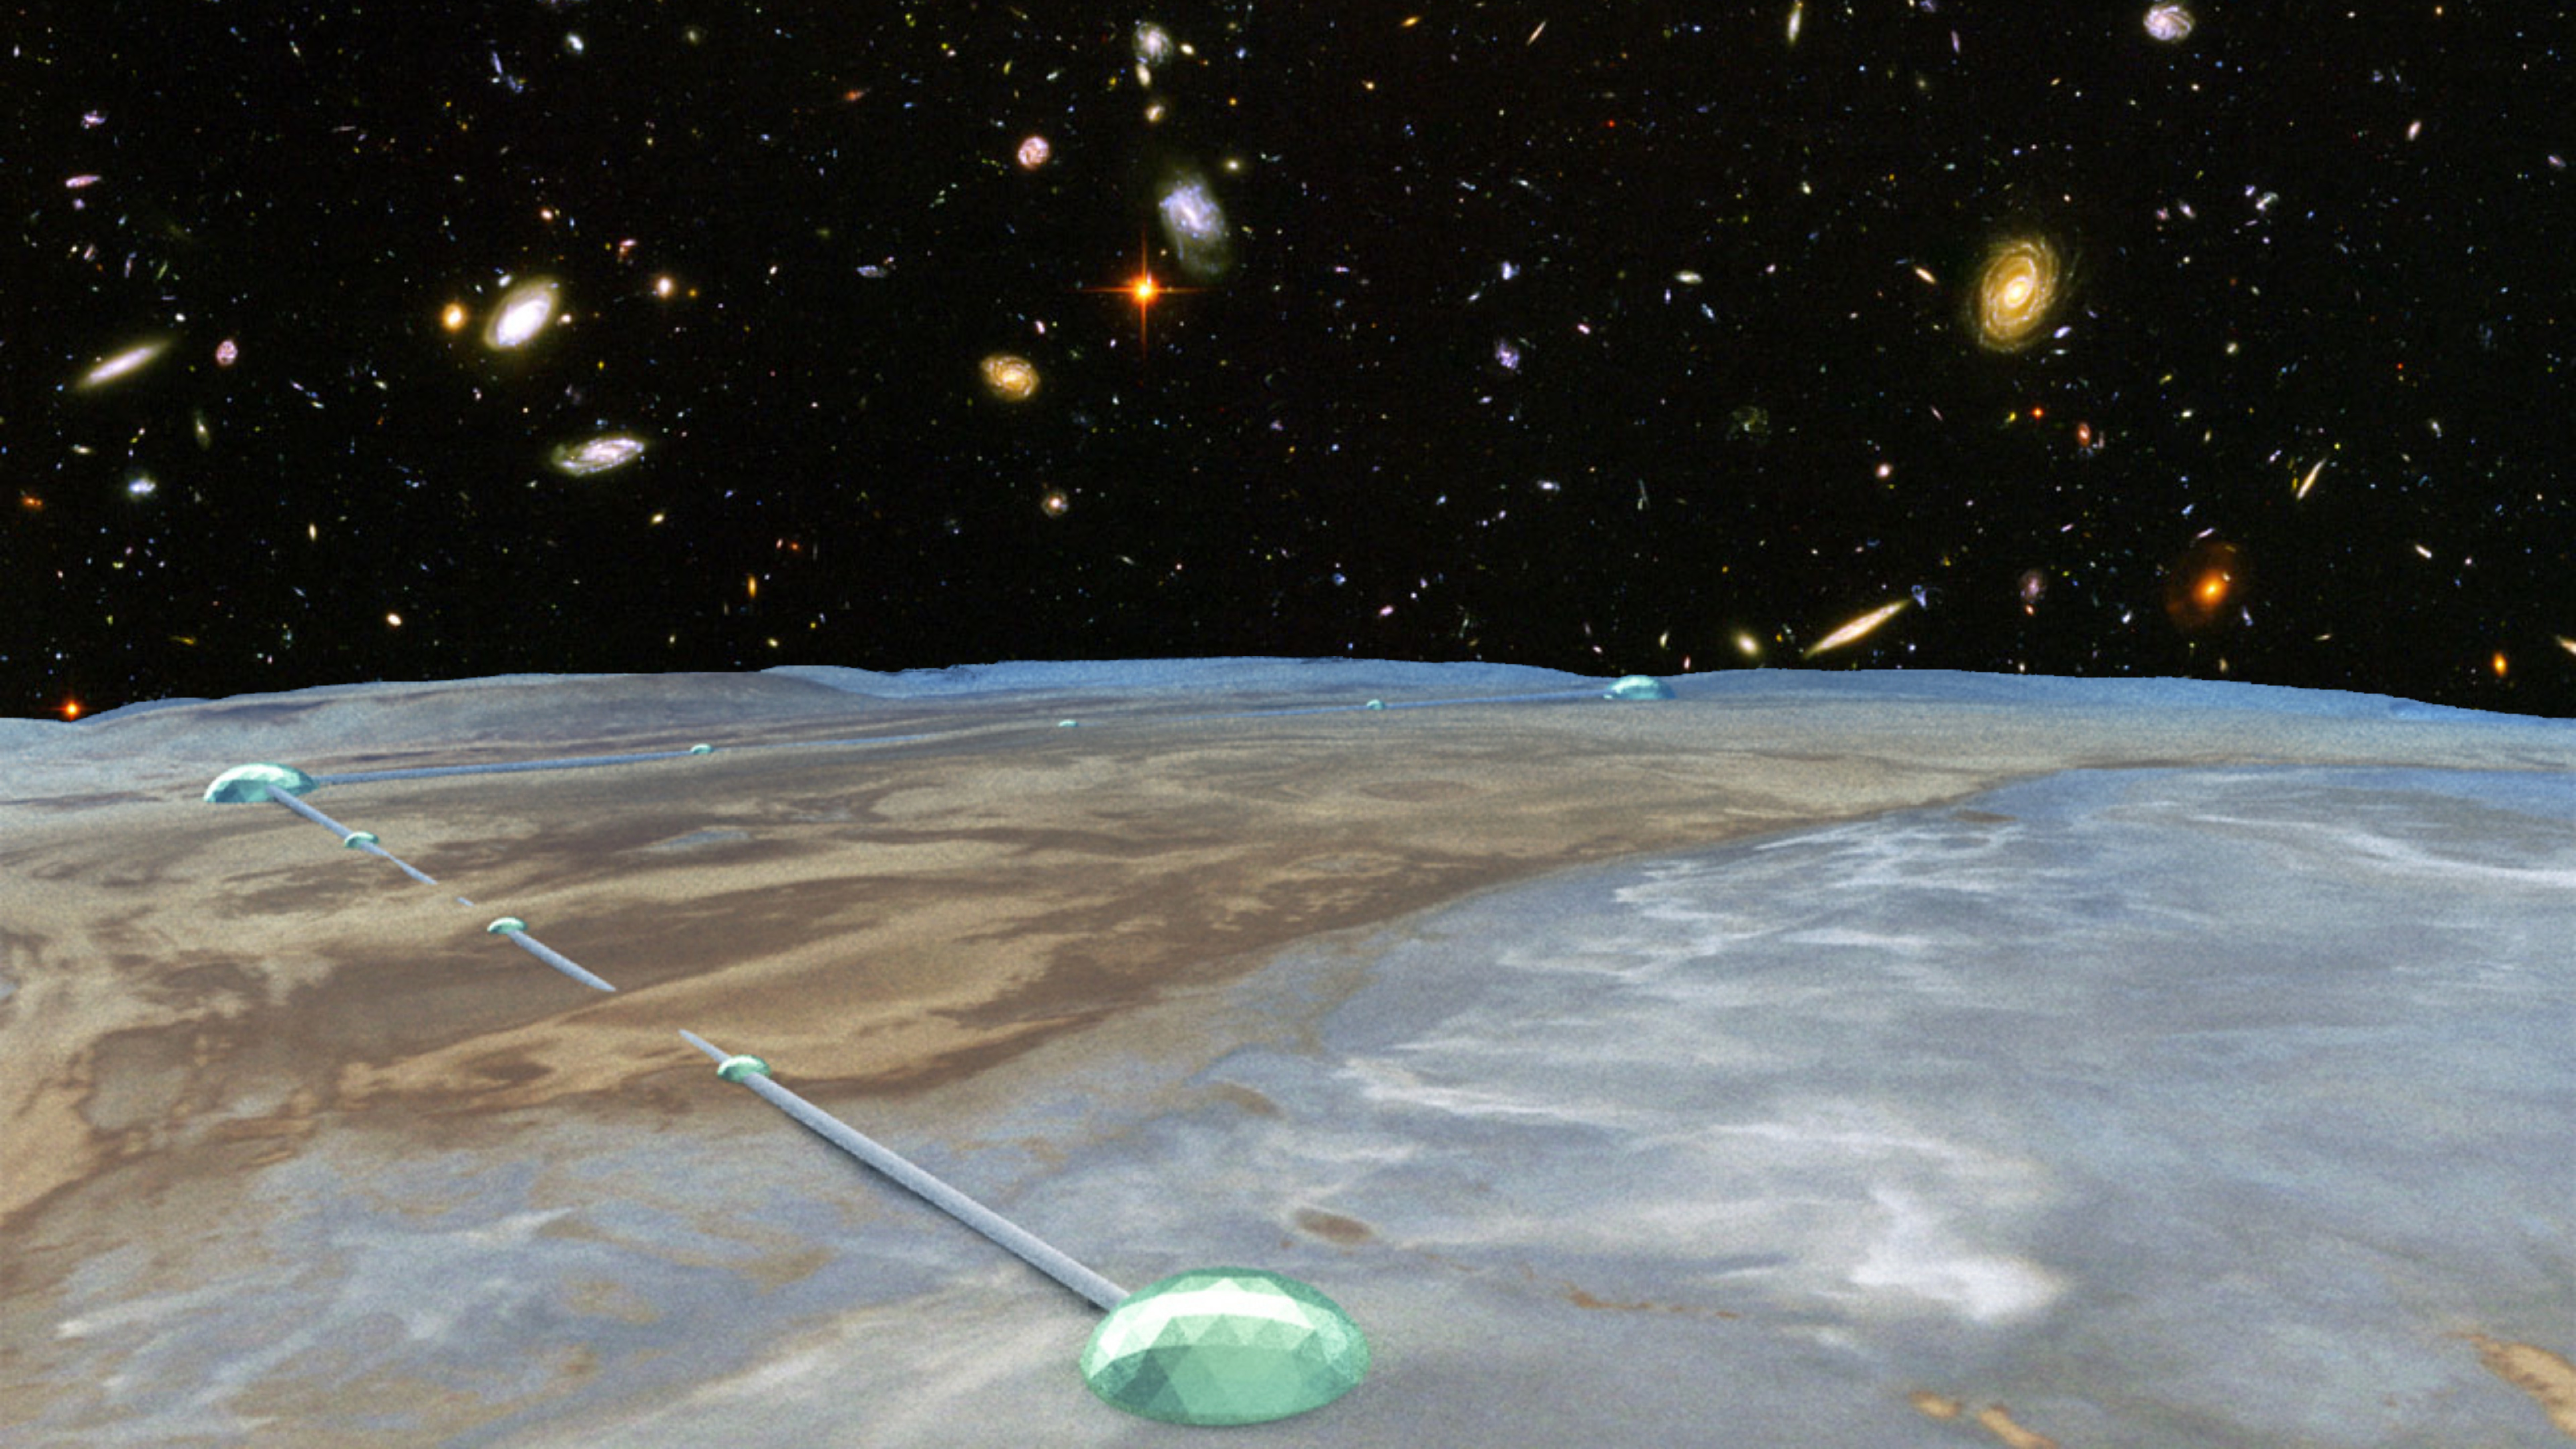
\includegraphics[width=0.48\textwidth]{ce-hubble-deep-field-reduced.jpg}} 
\caption{Artists conception of the Einstein Telescope (right panel) and Cosmic Explorer (right panel) observatories.  ET is conceived to consist of three, V-shaped, underground interferometers, formed out of 10 km sides of an equilateral triangle, while  Cosmic Explorer is conceived to be an L-shaped, overground interferometer, with 40 km arms.}
\label{fig:3G}
%\end{tcolorbox}
\end{figure*}

\begin{itemize}
\setlength\itemsep{0.2em}
    \item unequivocal evidence that GWs travel essentially at the speed of light, posing a challenge for the dark-energy inspired modified theories of gravity \cite{Monitor:2017mdv, Ezquiaga:2018btd, Sakstein:2017xjx}; % (see, however, \cite{deRham:2018red}); 
    \item first measurement of the Hubble constant using binary neutron stars as standard sirens to measure the luminosity distance to the host galaxy \cite{Abbott:2019yzh, Hotokezaka:2018dfi};  
    \item first GW measurement of the radius of neutron stars and constraints on the equation of state of ultra dense nuclear matter \cite{Abbott:2018wiz};  
    \item facilitating the first observation of a kilonova and identifying neutron star mergers as prolific sites for the production of heavy elements \cite{GBM:2017lvd};  
    \item solving one of the long lasting questions in astronomy by proving that binary neutron star mergers are progenitors of short, hard gamma-ray bursts \cite{GW-GRB170817};
    \item  discovery of a new class of \emph{heavy} black holes of masses in excess of $50\,M_\odot$ (GW150914 and GW170729) \cite{LIGOScientific:2018mvr, Chatziioannou:2019dsz}, in particular black holes in the pair-instability mass-gap (GW190521 \cite{}),  challenging astrophysical models of how they can form and their demographics;
    \item population properties of binary black holes and neutron stars that will be critical for understanding their formation and evolutionary models \cite{LIGOScientific:2018mvr}; 
    \item stringent bounds on the violations GR in the strong field regime of the theory \cite{TheLIGOScientific:2016src, Abbott:2018lct, Yunes:2016jcc}. 
    \item detection, for the first time, of the \emph{octupole} radiation in binary black holes with large mass asymmetries as in GW190412 \cite{LIGOScientific:2020stg} and GW190814 \cite{};
\end{itemize}

\subsection*{\bf Observatories of the Future}

Over the next few years Advanced LIGO and Virgo will reach their design sensitivities, followed by upgrades (termed A+ and V+) that will witness a factor of 3 increase in the detection rate. The LIGO-Virgo network will be enhanced by additional detectors, KAGRA in Japan, which is currently being commissioned, and LIGO-India in India, whose construction just began. 

Beyond the ``advanced-plus" era, several concepts are currently being discussed. {\em LIGO-Voyager} aims to further enhance the sensitivity of current LIGO facilities using cryogenic technology, new mirrors and higher power lasers \cite{Adhikari:2019zpy}, with a factor of xxx coverage in volume compared to advanced detectors.  The design study for the European {\em Einstein Telescope} began in 2008 and is currently the most mature concept for a future facility. It would be an underground observatory, housing three V-shaped detectors in the form of an equilateral triangle of 10 km side length (cf.\,Fig.\,\ref{fig:3G}, left panel) \cite{Punturo:2010zz}. In the US, the National Science Foundation has funded the {\em Horizon Study} of {\em Cosmic Explorer} (Fig.\,\ref{fig:3G}, right panel) \cite{CE}, with the goal of identifying the sensitivity requirements of a new facility that meets well-defined and unique science capabilities (see below).  In Australia NEMO is a new idea for a detector to target post-merger binary neutron star signals at $\sim$ kHz frequencies \cite{}. 

\begin{figure}[h]
    \centering
    \fbox{\includegraphics[width=0.45\textwidth]{horizon_donut_nsbh_Aplus_Voy_CE2_ET_dark_black.pdf}}
    \caption{Redshift reach of future observatories (assumed to be at the center of the diagram) for binary neutron stars (NS-NS), neutron star-black hole binaries (NS-BH) and binary black holes (BH-BH). Next generation observatories can push the horizon out to dark ages when the Universe was only a few hundred million years (Graphic: Evan Hall).}
    \label{fig:donut}
\end{figure}

\begin{figure*}
%\begin{tcolorbox}[standard jigsaw, colframe=ocre, colback=ocre!10!white, opacityback=1.0, coltext=black,title=\sc Science Goals for Next Generation Ground-Based Detectors]
 \begin{tcolorbox}[standard jigsaw,colframe=gray, colback=black!10!cyan, opacityback=0.1, coltext=black, title=\sc Box 1: Science Goals for Next Generation Ground-Based Detectors]

\begin{minipage}{0.45\textwidth}
\fbox{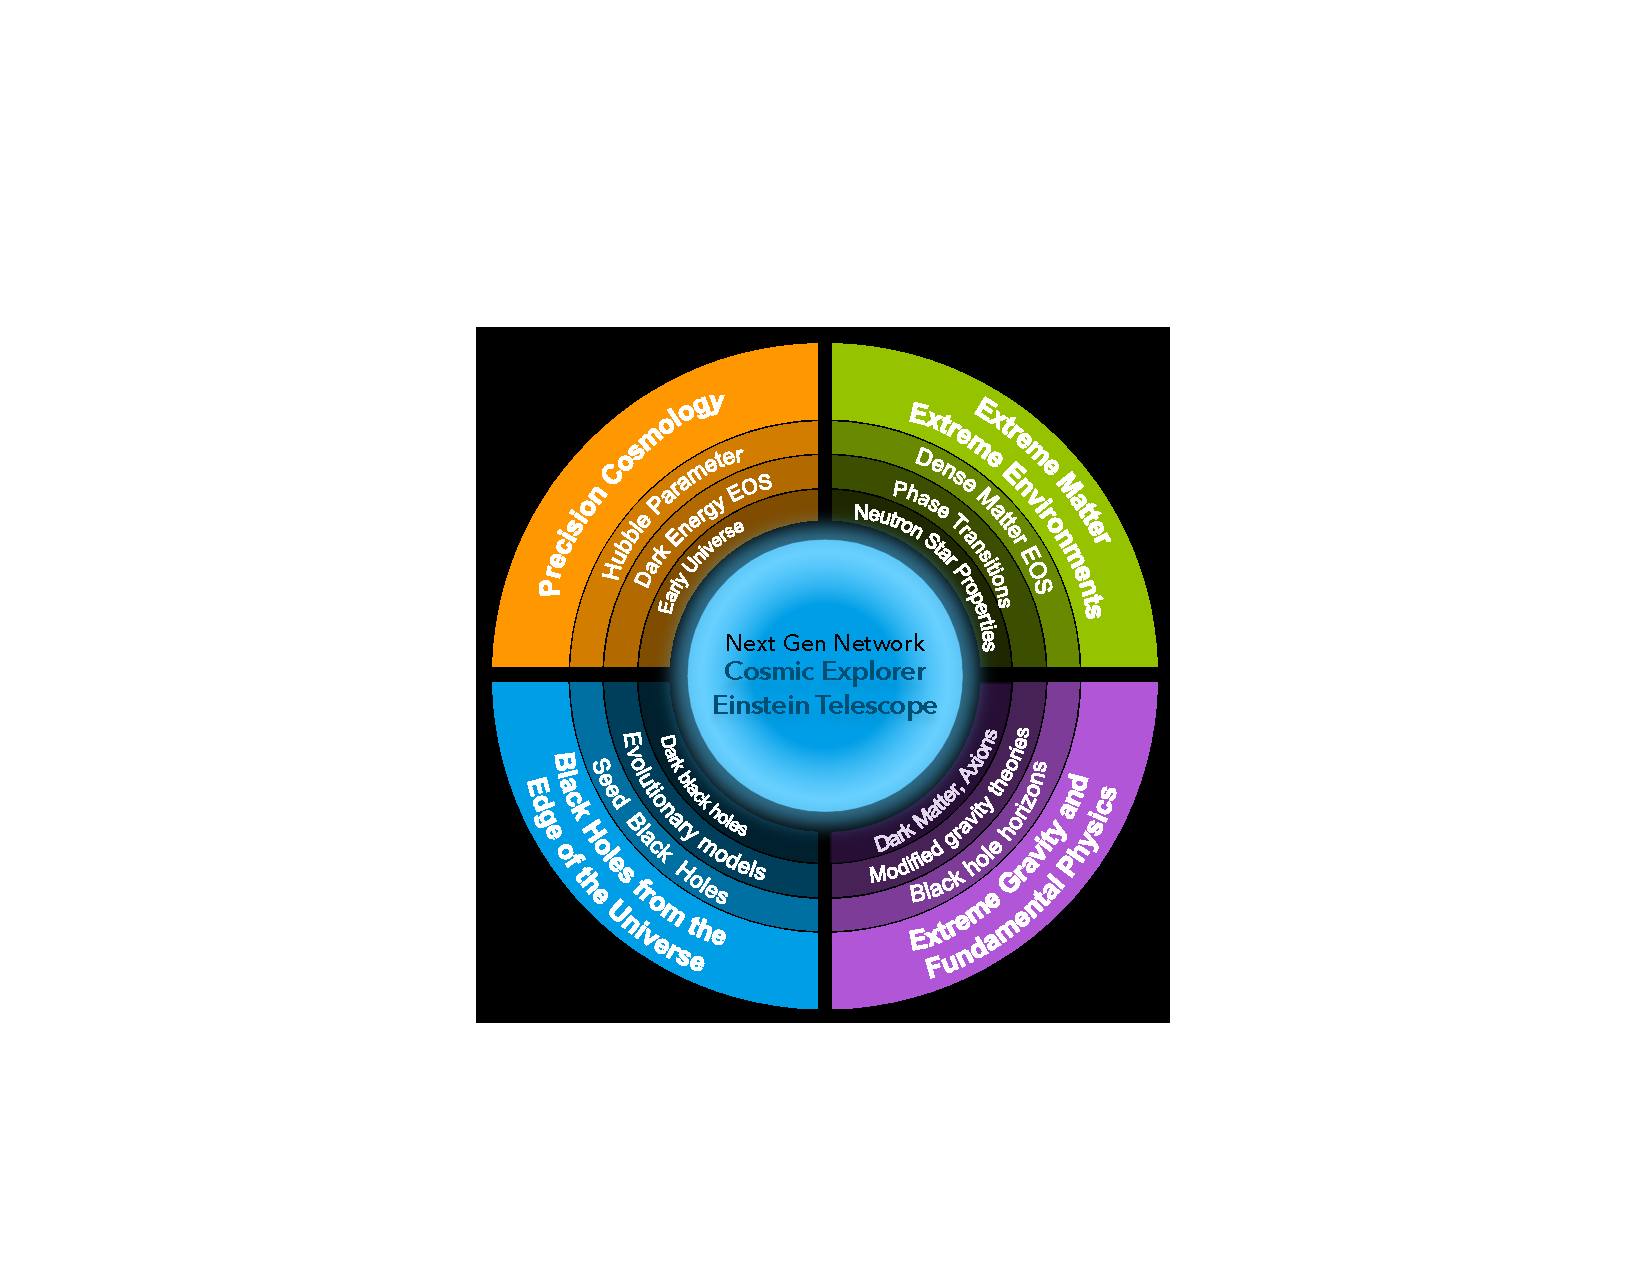
\includegraphics[width=1.05\textwidth]{3G-Science-Goals.pdf}}
\end{minipage}
\hfill
\begin{minipage}{0.50\textwidth}
\begin{itemize}
\item[] Future generations of ground-based gravitational-wave observatories will tackle fundamental questions on the nature of matter and spacetime. The adjacent \emph{Science Dial} summarizes the main science themes that can be uniquely explored with such observatories.
\item[$\odot$] Determine the equation-of-state of highest density matter and signature of quark-hadron phase transition.
\item [$\odot$]Explore the nature of dynamical spacetimes, detect dark matter around black holes and test general relativity and modified gravity theories. 
\item [$\odot$]Study the origin of seed black holes that support the formation of galaxies like the Milky Way and power quasars.
\item [$\odot$] Enable precision measurement of cosmological parameters such as the dark energy, and phase transitions in the early Universe. 
\end{itemize}
\end{minipage}
\end{tcolorbox}
\end{figure*}

The global instrument research community is exploring a wide range of new technologies for
 the next generation of observatories.
These range from relatively near-term enhancements of existing technology,
 such as larger mirrors and suspensions, improved vibration isolation systems and higher-power lasers,
 to new materials and coatings for low-temperature operation.
Low-temperature interferometers with silicon optics and 2\,$\rm \mu m$ lasers appear promising,
 but offer many challenges and open questions.
These include the production of high-quantum efficiency photo detectors, low-loss optical isolators,
 low-absorption amorphous silicon coatings and large single-crystal silicon optics, just to name a few.

\subsection*{\bf Next Generation GW Astronomy}
Over the next two decades gravitational-wave observatories will take the leap to survey the entire Universe for binary black holes and detect binary neutron stars from epochs when star formation was still in its infancy (see Fig.\,\ref{fig:donut}). It is difficult to overstate the discovery potential of such observatories but if past experience with classical astronomy is any guide we can be confident that gravitational-wave astronomy will not only unravel many of the outstanding mysteries but also discover new physics and astronomical phenomena.

Unique and wide ranging science questions that can be addressed by the next generation observatories is summarized in Box 1. The topics vary from foundational questions in fundamental physics, such as the nature of spacetime and the state of ultra dense matter, to the biggest questions in astronomy, such as the origin of supermassive black holes that support the formation of galaxies. We will describe a sample of these questions in some detail below.

\noindent \paragraph{Extreme gravity \& fundamental physics.}
GWs emanate from regions of strong gravity and large curvature, carrying uncorrupted information from their sources (\ref{fig:TGR-EM}, left panel). Imprint in the signal is the nature of the gravitational field, characteristics of the sources and the physical environment in which they reside. Their observation in a 3G network can subject GR to the most stringent tests, help explore violations of the theory in strong fields. For example, GW observations could reveal new particles and fields that breach the strong equivalence principle, discover violations of the Lorentz invariance, or detect extra polarizations of GWs. One might also infer the signature of quantum gravity, e.g., pseudo-scalar configurations that violate parity, or birefringence of the waves propagating over great distances.  Ultra-light Bosonic fields proposed in certain extensions of the Standard Model could be detected via their effect on the orbital dynamics of black hole binaries and spin properties of black holes.

Black holes are the most compelling explanation for the companion stars in binary coalescences discovered by LIGO and Virgo. The tell tale signature of their presence would be seen in the quasi-normal mode spectrum of the merger remnant, whose frequencies and damping times should depend only on two parameters: the remnant's mass and spin. Signature of additional degrees of freedom would be seen as inconsistency in the remnant's parameters determined by the different modes of gravitational waves. In certain modified gravity theories black holes could mimic the quasi-normal mode spectra, but they could emit additional signals in the form of echoes of the ingoing radiation reflected from their surface, which could be observable in the 3G network.



\noindent \paragraph{Extreme matter \& extreme environs.}
Neutron stars are the densest objects in the Universe with magnetic fields as large as billions of Tesla. Six decades after their first discovery we still lack a proper understanding of the equation of state of their deep cores and the origin of their large magnetic fields. Neutron stars in a binary are subject to the tidal fields of their companions. The magnitude of the tidal deformation depends on the state of matter in their dense cores and will be imprint in the GWs emitted is the signature of this deformation.  Furthermore, the merger could leave behind a short-lived, hyper-massive neutron star. Gravitational radiation from the remnant from could reveal unknown physics in the state of ultra-high density matter, e.g. phase transition from hadrons to quark-gluon plasma.

The origin of heavy elements in the Universe has been a long-standing problem. Electromagnetic observation of GW170817 provided irrefutable evidence that binary neutron star mergers are sites of production of lanthanides and other heavy elements. Next generation observatories will provide the unique opportunity to electromagnetically follow-up thousands of mergers, a number that is required to confirm if the abundance of heavy elements in the Universe can be explained by mergers alone or if other production channels are necessary.

\noindent \paragraph{Black Holes from the Edge of the Universe.}
There is growing evidence that all galaxies host massive black holes of 
at their centers whose masses (found to be in the range $\sim 10^6$--$10^{10}$ solar mass) are largely correlated with the size of the galaxy. however, we do not know the origin of these black holes nor how they got to be so huge. one of the models posits that they were initially seeded by heavy stellar-mass black holes found by gw observations and grew by hierarchical merger. an alternative scenario supposes that massive black holes formed by the direct collapse of massive gas clouds and would require fewer mergers to grow big. an intriguing third possibility is that these black holes formed in the primordial universe that then led to the collapse of dark matter and baryons around them triggering the formation of galaxies.   Next generation observatories will chart a complete census of stellar mass black holes up to an epoch when the Universe was just a few hundred million years old assembling its first stars and hence test the hierarchical merger model.

Since LIGO's first discovery, the origin of black hole binaries has been a subject of great debate. So far, it has not been possible to confirm any of a host of models that have been invoked as their origin.  Evolutionary scenarios include formation of black hole binaries as the end product of isolated, massive, stellar binaries or formation of black holes in globular, nuclear or stellar clusters that then sink in to the center of the cluster where they pair up with other black holes that have similarly sunk in.  A third scenario stems from the idea that dark matter is essentially primordial black holes that form the halo of the galaxy and it is their random pairing and merger that we now observe. Once again future observatories network will pin down the population properties of black holes that could be used to determine the principal formation channels and resolve fundamental questions about their origin. 


\begin{figure*}
\fbox{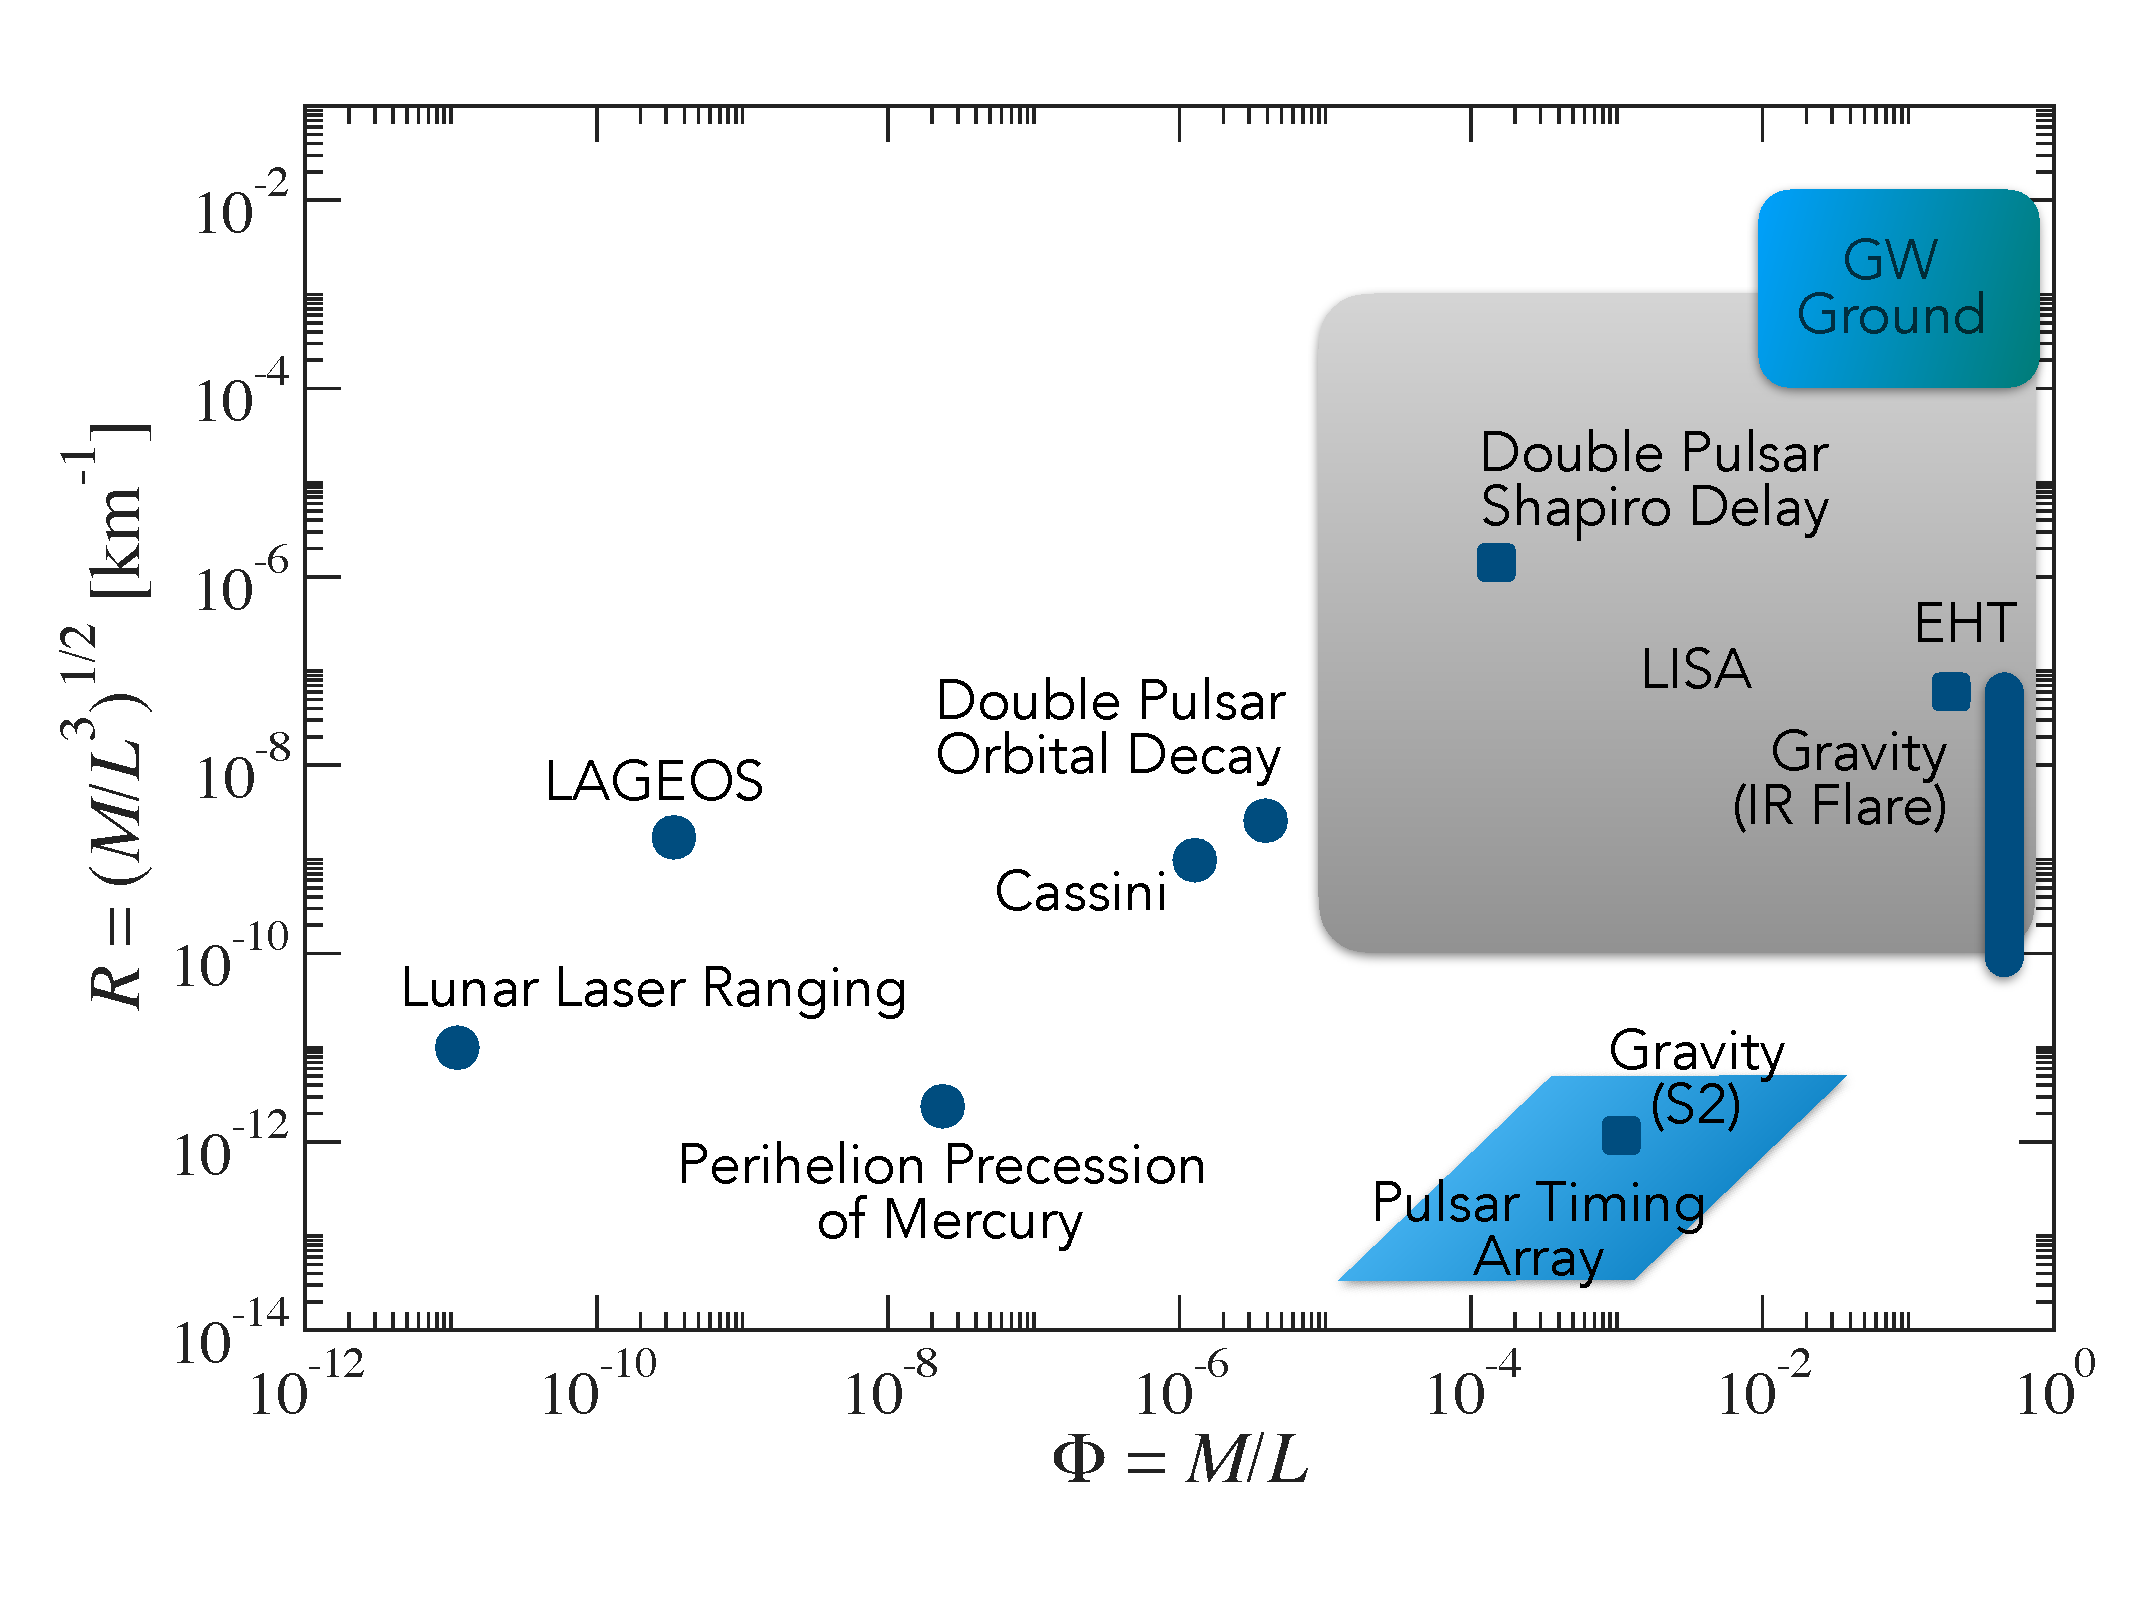
\includegraphics[width=0.5\textwidth]{ToG2.pdf}}
\fbox{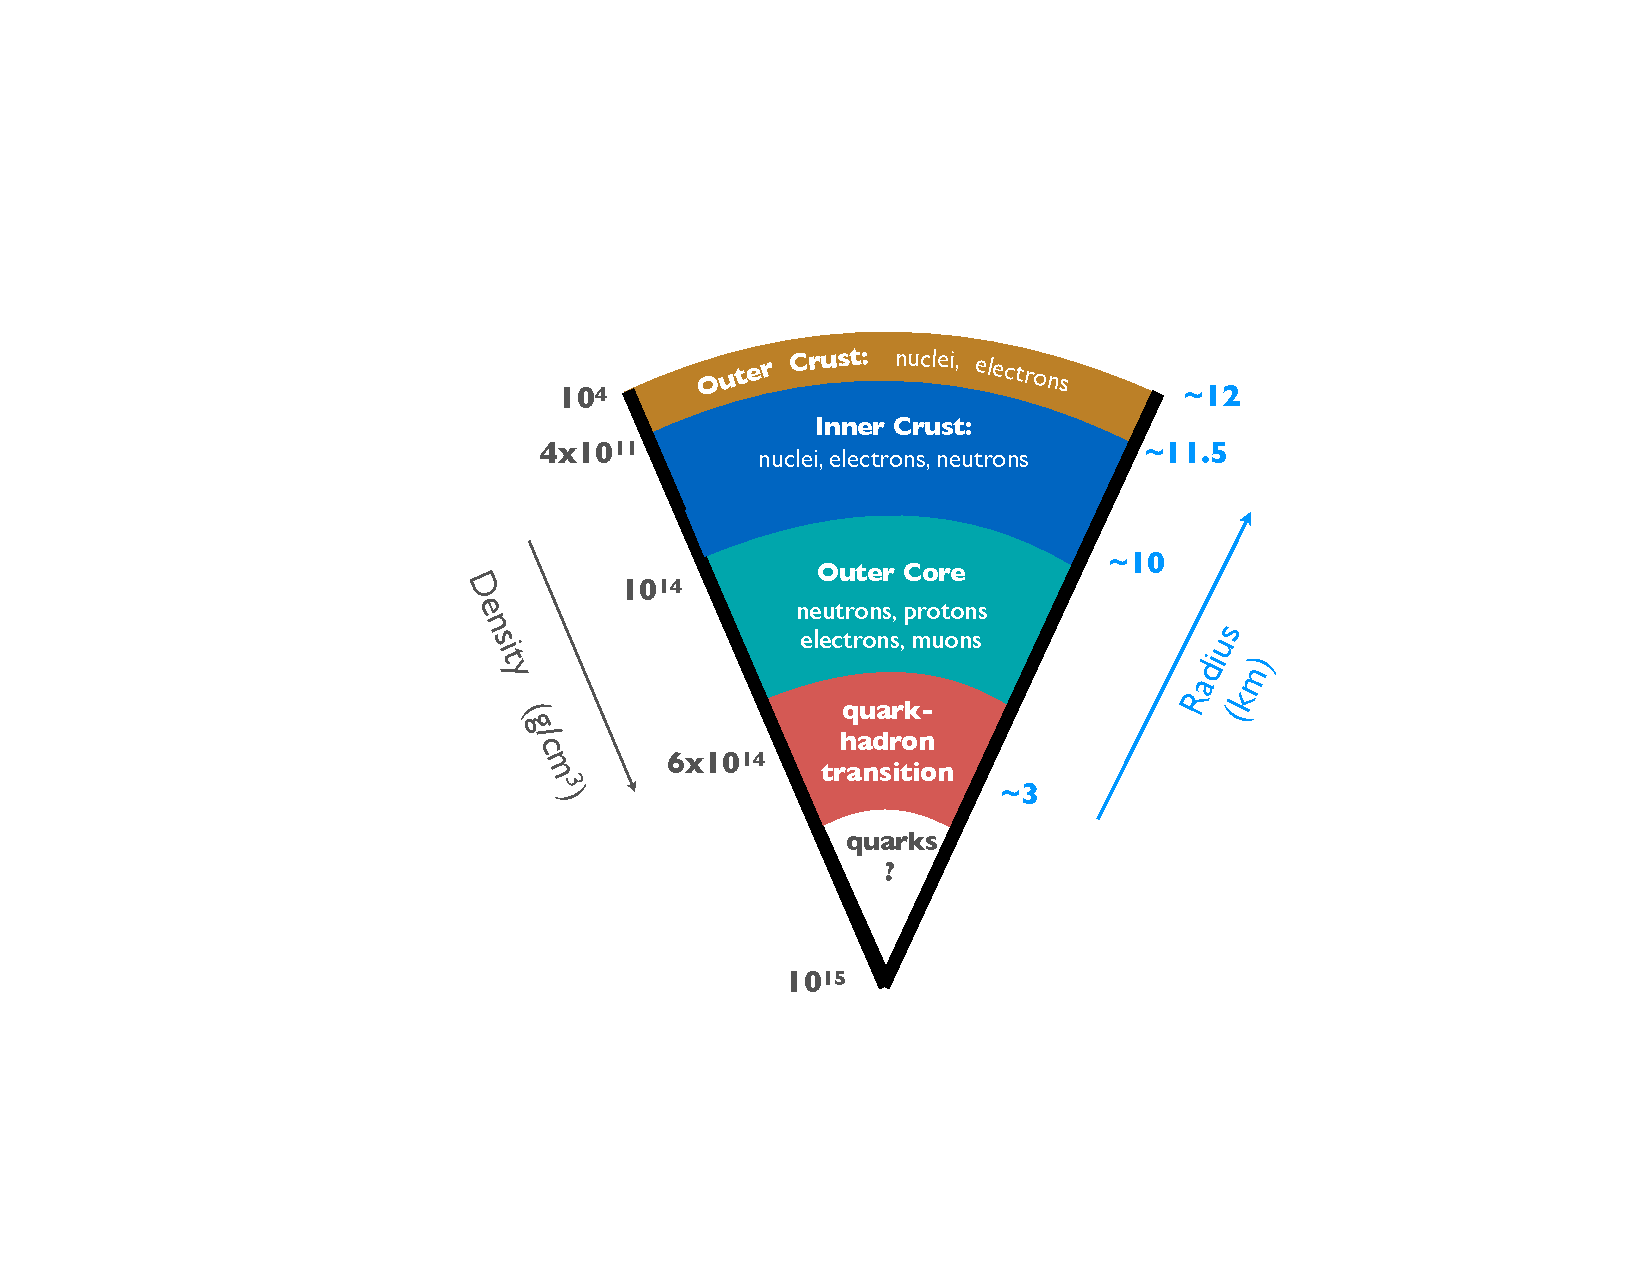
\includegraphics[width=0.415\textwidth]{NS_Profile.pdf}}
\caption{The left plot shows the curvature scale $R$ plotted as a function of dimensionless gravitational potential or compactness (in $c=G=1$ units) and right hand diagram shows the structure of ultra-dense matter in neutron star cores. Future ground-based GW observatories will probe the largest curvature scales nd compactness but also the state of most extreme matter, in particular if matter at ultra high densities undergoes a phase transition to quark-gluon plasma. (Right panel: Sanjay Reddy).}
\label{fig:TGR-EM}
\end{figure*}

\noindent \paragraph{Cosmology and Early History of the Universe.}
Big bang cosmology is largely consistent with GR but the accelerated expansion of the Universe in its recent history cannot be explained by the theory, indicating either its failure or the presence of exotic form of matter-energy density. Observations on galactic to cosmological scale provide unequivocal indirect evidence for the presence of weakly interacting dark matter, but none has been directly detected in spite of concerted efforts over the past six decades. Future GW observatories could detect various forms of dark matter, including axionic and other dark matter fields around black holes and neutron stars. 

The geometry and expansion rate of the Universe can be inferred by measuring distances and redshifts to sources at cosmological distances of several billion light years.  GWs from the inspiral and merger of compact binaries can be used to infer the luminosity distance to their sources without the need to calibrate them with standard candles. This is because the orbital dynamics of binary black holes and neutron stars is largely determined by Einstein's theory of gravity.

A handful of parameters, e.g. masses and spins of the companion stars, precisely control the pattern of the emitted GWs. The amplitude of that pattern is fixed by the distance to the source, sky position and orientation of the source relative to a detector, which can be inferred with a network of three or more non-collocated detectors.  This contrasts with the dynamics of other astrophysical systems, such as supernovae, that require detailed modelling of their composition and environment, making it extremely hard to predict the spectral energy density of electromagnetic waves with any precision.  With a population of compact binary mergers observed with 3G detectors, and their redshifts obtained by follow up electromagnetic observations, it will be possible to accurately measure cosmological parameters such as the Hubble parameter, dark matter and dark energy densities and the equation of state of dark energy, giving a completely independent and complementary measurement of the dynamics of the Universe.

Stochastic gravitational waves are expected to be produced in the early Universe. As the Universe cools from its primeval hot and dense phase it undergoes several phase transitions that are expected to generate a gravitational-wave background. Detection of such a background would dramatically transform our state of knowledge of the underlying particle theory at energy scales that will never be accessible in terrestrial accelerators. Defects, such as cosmic strings, associated with symmetry breaking and phase transitions could also be source of stochastic or deterministic sources. The landscape of cosmic sources of gravitational waves, while uncertain, is a high-risk high-reward endeavor to pursue in the era of 3G detectors.

\noindent \paragraph{Sources at the Frontier of Observations}
The physics of supernovae, stellar glitches and quakes is an open problem in astrophysics. Many of these systems will generate gravitational waves that will be detectable with 3G observatories at distances of several million light years for supernovae and within the galaxy for quakes in pulsars and glitches in magnetars.  Multimessenger observations of these systems with the 3G network, enhanced by EM and neutrino observatories, will allow us to probe extreme astrophysics and address key questions that have hindered progress in our understanding of the mechanism behind stellar explosions.

\subsection*{Summary}
LIGO and Virgo detections have ushered in the new era of multi-messenger physics and astronomy.  GW astronomy can be used for understanding not just the sky but also to test general relativity in dynamical spacetimes, to gain insights into the nature of matter under extreme physical conditions of gravity, density, and pressure, to discover the nature of dark matter, dark energy and other exotic objects, to explore the nature of most violent processes in the Universe, to study the formation and evolution of stellar mass black holes throughout the Universe and to probe the physics of the early history and evolution of the Universe. The science case for building a new generation of GW observatories that can probe deep into the cosmos and observe a variety of different processes is immensely rich and massively rewarding. 


\bibliographystyle{h-physrev4}
\bibliography{biblio,Ref_list}

\end{document}

\begin{figure*}
\begin{tcolorbox}[standard jigsaw, colframe=gray, colback=black!10!cyan, opacityback=0.1, coltext=black, title=\sc What are gravitational Waves]
% \begin{minipage}{0.40\textwidth}
\begin{itemize}
    \item [$\odot$] In general relativity the spacetime metric plays the role of the potential. Unlike Maxwell's theory, however, the first derivatives of the metric, representing the acceleration field, are not physical; they can all be set to zero by a suitable choice of gauge. This is due to the physical consequence of the {\em principle of equivalence} because of which gravity can be removed locally. The second derivatives of the metric, representing the tidal field, are the true physical degrees of freedom and they capture the curvature of spacetime. Thus, wave-like solutions to the potential translate to wave-like behavior of the spacetime curvature and hence gravitational waves are ripples in the very fabric, that is the curvature, of spacetime.

    \item[$\odot$] Gravitational waves are transverse, travel at the speed of light and have two polarization states. The diagram shows the effect of a sinusoidal wave of amplitude $h_0$ and frequency $\omega$ on a ring of free test masses (white dots) in the transverse plane. The ring is deformed into an ellipse by the tidal action of the waves (shown by green and red arrows), stretched and squeezed in orthogonal directions which are reversed after half the wave-period. The deformation due to the two polarizations are separated by an of $\pi/4$ radians since (in general relativity) gravitational waves are helicity 2.\\
\end{itemize}
% \end{minipage}
% \begin{minipage}{0.48\textwidth}
\centering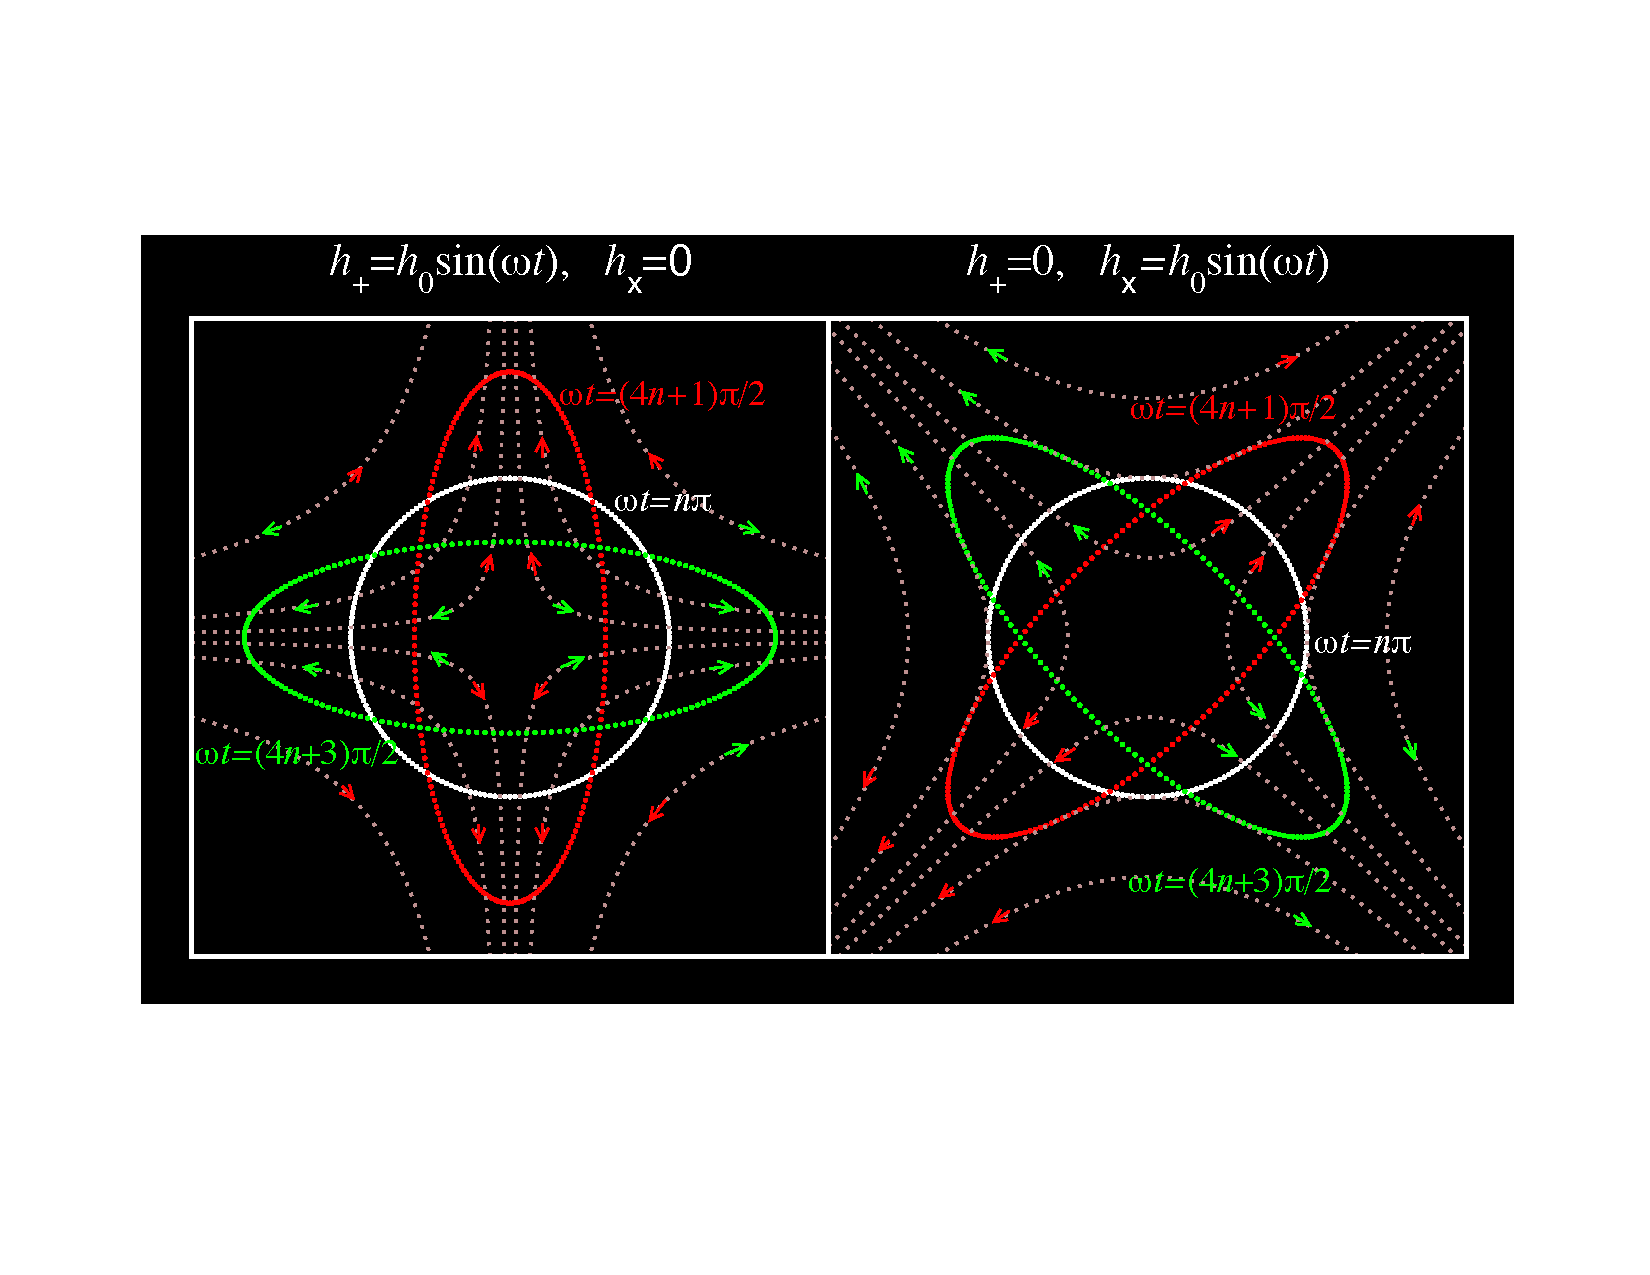
\includegraphics[width=0.8\textwidth]{polarization.pdf}
% \end{minipage}
\end{tcolorbox}
\end{figure*}


Gravitational waves are ripples in the geometry of spacetime produced by accelerating masses such as a pair of black holes orbiting about each other. Indeed, an orbiting pair of black holes would lose energy into gravitational waves, spiral in and collide at half the speed of light. In the final epochs before they merge, they would momentarily appear more luminous in gravitational waves than the electromagnetic radiation of all the stars in the Universe.

% As gravitational waves propagate they cause tidal deformation of the proper distance between free test masses with the same oscillation frequency as the passing wave (see Box 1). Laser interferometers take advantage of this differential change in length caused by the waves to detect them. Even for the most catastrophic events the change length in a km sized interferometer is minuscule, thousands of times smaller than the diameter of a proton. Thus, LIGO's discovery in 2015 was a new record in precision measurement and ushered in a new era to explore the hidden mysteries of the Universe. It was now possible to observe the Universe with a new cosmic  discover new physics that might explain some of the current crisis in fundamental physics and cosmology.

Gravitational waves emanate from regions of strong gravity and their sources have stupendously large spacetime curvature.  There is simply no other tool available to probe such regions of spacetime. 

% This was a triple discovery from an experiment that was only at the beginning of its operation: first direct observation of gravitational waves, first discovery of binary black holes, and first ever record of the formation of a black hole. 